\section{Validação}

Com o objetivo de testar a implementação e proposta de valor da ferramenta, é feito uma pesquisa comparativa focando no impacto do seu uso em relação a mudanças de fluxo de dados pelo servidor que afetam o contrato de acesso.

Para isso será desenvolvido um ambiente de validação onde dois clientes realizam três consultas em serviço através de uma API REST. Um deles fazendo o uso da ferramenta e o outro não. Após disso, será aplicado uma série de mudanças no serviço que afetam o fluxo de dados para que assim, possa ser analisado o impacto e resultado através das  variáveis coletadas. \\

\textbf{Estrutura de dados (JSON)} \\

Foi escolhido trabalhar com um escopo de serviço chamado SWAPI, bastante utilizado para análise de implementações de estilos de arquitetura e linguagens de programação. Nele, são descritos seis entidades e seus respectivos relacionamentos.

\begin{figure}[H]
  \centering
  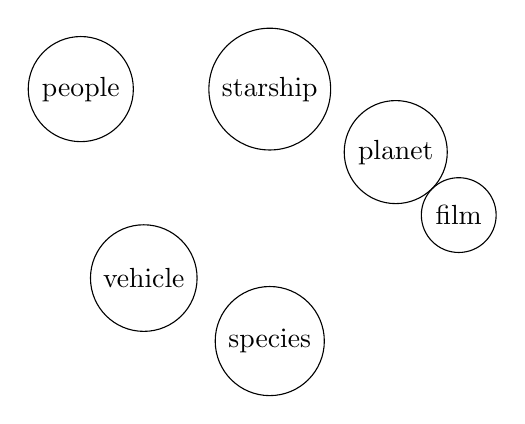
\begin{tikzpicture}
    [scale=.8,auto=left,every node/.style={circle,draw}]
    \node (film) at (3,7)  {film};
    \node (people) at (-3,9)  {people};
    \node (starship) at (0,9) {starship};
    \node (vehicle) at (-2,6)  {vehicle};
    \node (species) at (0,5)  {species};
    \node (planet) at (2,8)  {planet};
  \end{tikzpicture}
  \caption{Entidades SWAPI}
\end{figure}

\textbf{Consultas e respostas esperadas} \\

Com o propósito de explorar cada ponto de acesso e estrutura de dados do serviço SWAPI, foram pensadas em três perguntas de média complexidade onde envolvessem ao menos três das entidades da API. Para cada pergunta existe apenas uma resposta certa, onde sua lógica é baseada em campos das estruturas de dados remotas.

\begin{enumerate}
\item Qual o nome do filme no qual aparece mais personagens oriundos de um planeta deserto? R: "Revenge of the Sith"

\begin{figure}[H]
  \centering
  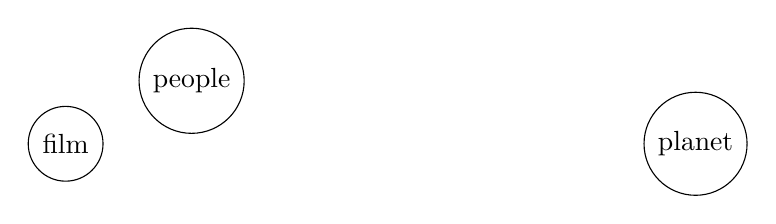
\begin{tikzpicture}
    [scale=.8,auto=left,every node/.style={circle,draw}]
    \node (film) at (0,8)  {film};
    \node (people) at (2,9)  {people};
    \node (planet) at (10,8)  {planet};
  \end{tikzpicture}
  \caption{Entidades envolvidas na primeira pergunta}
\end{figure}

\item Qual o nome da espécie predominante entre os habitantes do planeta "Tatooine"? R: "Droid"

\begin{figure}[H]
  \centering
  \begin{tikzpicture}
    [scale=.8,auto=left,every node/.style={circle,draw}]
    \node (people) at (2,9)  {people};
    \node (specie) at (8,5)  {specie};
    \node (planet) at (10,8)  {planet};
  \end{tikzpicture}
  \caption{Entidades envolvidas na segunda pergunta}
\end{figure}

\item Qual o nome do personagem que mais pilota espaçonaves e veículos durante o filme "A New Hope"? R: "Chewbacca"

\begin{figure}[H]
  \centering
  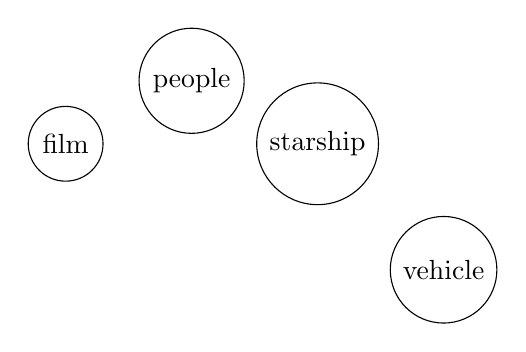
\begin{tikzpicture}
    [scale=.8,auto=left,every node/.style={circle,draw}]
    \node (film) at (0,8)  {film};
    \node (people) at (2,9)  {people};
    \node (starship) at (4,8) {starship};
    \node (vehicle) at (6,6)  {vehicle};
  \end{tikzpicture}
  \caption{Entidades envolvidas na terceira pergunta}
\end{figure}

\end{enumerate}

\textbf{Mudanças no fluxo de dados} \\

É proposto quatro tipos de mudanças no fluxo de dados para quebra de contrato, onde cada mudança testa a capacidade da ferramenta em a adaptar a comunicação através da atualização dos metadados do serviço.

\begin{enumerate}
\item Mudança no endereço de ponto de acesso.
\item Mudança no nível de estrutura de resposta.
\item Adição de ponto de acesso otimizado.
\item Remoção de ponto de acesso deprecado.
\end{enumerate}

\textbf{Variáveis} \\

É descrito cinco variáveis para análise dos testes de validação. Todos são quantitativas e coletadas no cliente após o processo de mudança.

\begin{table}[H]
  \centering
  \begin{tabular}{|c|c|c|}
    \hline
    Variável & Unidade & Tipo \\
    \hline
    Porcentagem de acerto & \% & Quantitativa \\
    \hline
    Tamanho de resposta & kb & Quantitativa \\
    \hline
    Número de requisições & inteiro & Quantitativa \\
    \hline
    Tempo de busca de metadados & ms & Quantitativa \\
    \hline
    Tempo de processamento & ms & Quantitativa \\
    \hline
  \end{tabular}
  \caption{Variáveis de análise}
\end{table}

 
 
 
 
 
 

 
